\documentclass{article}
\usepackage[utf8]{inputenc}
\usepackage{hyperref}
\usepackage[letterpaper, portrait, margin=1in]{geometry}
\usepackage{enumitem}
\usepackage{amsmath}
\usepackage{booktabs}
\usepackage{graphicx}
\usepackage{hyperref}
\usepackage{titlesec}

\hypersetup{
colorlinks=true,
    linkcolor=black,
    filecolor=black,      
    urlcolor=blue,
    citecolor=black,
}

  
\title{Economics 7103 - Homework 2}
\author{Ana Mazmishvili}
\date{ January 29, 2024 }
  
\begin{document}
  
\maketitle 

\section*{Python}
\textbf{Note:} \textit{I asked Afi to help me with the Python code only. That's why I will follow similar steps as he did with small modifications. }

\subsection*{Question 1.1}
\textbf{Response:} Randomization worked which is demonstrated by comparison across control and treatment groups that indicates statistical balance in observables. Column 3 presents the differences in means and the standard errors of the differences in brackets. The differences are small and in case of electricity consumption statistically significant.

\begin{table}[ht]
    \centering
    \input{homework 2/output/table/SummaryTablePy}
    \caption{Summary Statistics for the treated and control groups.}
    \label{tab:my_label}
\end{table}


\subsection*{Question 1.2}

\begin{figure}[ht]
    \centering
    \includegraphics[scale = 0.7]{homework 2/output/figure/densityplotpy.pdf}
    \caption{Kernel density plots of the electricity use for treated group and control group.}
    \label{fig:hist}
\end{figure}

\subsection*{Question 1.3}

\section*{Stata}

\subsection*{Question 2.1}


\begin{table}[ht]
    \centering
    \input{homework 2/output/table/summarytable}
    \caption{Summary statistics produced using Stata}
    \label{tab:my_label}
\end{table}

\subsection*{Question 2.2}

\begin{figure}[ht]
    \centering
    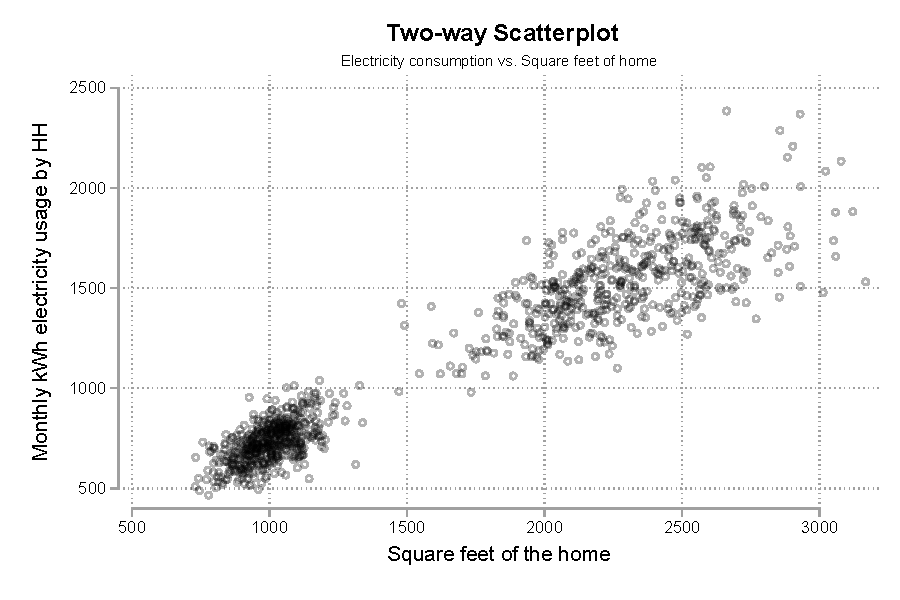
\includegraphics[scale = 0.7]{homework 2/output/figure/scatterplot.pdf}
    \caption{Scatterplot with electricity consumption and square feet of home}
      \label{fig:scatter}
\end{figure}

\subsection*{Question 2.3}
\begin{table}[ht]
    \centering
    \input{homework 2/output/table/robustOLS}
    \caption{OLS regression results using Stata}
     \label{tab:my_label}
  \end{table}




\end{document}